%  LaTeX support: latex@mdpi.com
%  In case you need support, please attach all files that are necessary for compiling as well as the log file, and specify the details of your LaTeX setup (which operating system and LaTeX version / tools you are using).

%=================================================================
\documentclass[agriculture,article,submit,moreauthors,pdftex]{mdpi}

% If you would like to post an early version of this manuscript as a preprint, you may use preprint as the journal and change 'submit' to 'accept'. The document class line would be, e.g., \documentclass[preprints,article,accept,moreauthors,pdftex]{mdpi}. This is especially recommended for submission to arXiv, where line numbers should be removed before posting. For preprints.org, the editorial staff will make this change immediately prior to posting.

%% Some pieces required from the pandoc template
\providecommand{\tightlist}{%
  \setlength{\itemsep}{0pt}\setlength{\parskip}{4pt}}
\setlist[itemize]{leftmargin=*,labelsep=5.8mm}
\setlist[enumerate]{leftmargin=*,labelsep=4.9mm}

\usepackage{longtable}

% see https://stackoverflow.com/a/47122900

%--------------------
% Class Options:
%--------------------
%----------
% journal
%----------
% Choose between the following MDPI journals:
% acoustics, actuators, addictions, admsci, aerospace, agriculture, agriengineering, agronomy, algorithms, animals, antibiotics, antibodies, antioxidants, applsci, arts, asc, asi, atmosphere, atoms, axioms, batteries, bdcc, behavsci , beverages, bioengineering, biology, biomedicines, biomimetics, biomolecules, biosensors, brainsci , buildings, cancers, carbon , catalysts, cells, ceramics, challenges, chemengineering, chemistry, chemosensors, children, cleantechnol, climate, clockssleep, cmd, coatings, colloids, computation, computers, condensedmatter, cosmetics, cryptography, crystals, dairy, data, dentistry, designs , diagnostics, diseases, diversity, drones, econometrics, economies, education, electrochem, electronics, energies, entropy, environments, epigenomes, est, fermentation, fibers, fire, fishes, fluids, foods, forecasting, forests, fractalfract, futureinternet, futurephys, galaxies, games, gastrointestdisord, gels, genealogy, genes, geohazards, geosciences, geriatrics, hazardousmatters, healthcare, heritage, highthroughput, horticulturae, humanities, hydrology, ijerph, ijfs, ijgi, ijms, ijns, ijtpp, informatics, information, infrastructures, inorganics, insects, instruments, inventions, iot, j, jcdd, jcm, jcp, jcs, jdb, jfb, jfmk, jimaging, jintelligence, jlpea, jmmp, jmse, jnt, jof, joitmc, jpm, jrfm, jsan, land, languages, laws, life, literature, logistics, lubricants, machines, magnetochemistry, make, marinedrugs, materials, mathematics, mca, medicina, medicines, medsci, membranes, metabolites, metals, microarrays, micromachines, microorganisms, minerals, modelling, molbank, molecules, mps, mti, nanomaterials, ncrna, neuroglia, nitrogen, notspecified, nutrients, ohbm, particles, pathogens, pharmaceuticals, pharmaceutics, pharmacy, philosophies, photonics, physics, plants, plasma, polymers, polysaccharides, preprints , proceedings, processes, proteomes, psych, publications, quantumrep, quaternary, qubs, reactions, recycling, religions, remotesensing, reports, resources, risks, robotics, safety, sci, scipharm, sensors, separations, sexes, signals, sinusitis, smartcities, sna, societies, socsci, soilsystems, sports, standards, stats, surfaces, surgeries, sustainability, symmetry, systems, technologies, test, toxics, toxins, tropicalmed, universe, urbansci, vaccines, vehicles, vetsci, vibration, viruses, vision, water, wem, wevj

%---------
% article
%---------
% The default type of manuscript is "article", but can be replaced by:
% abstract, addendum, article, benchmark, book, bookreview, briefreport, casereport, changes, comment, commentary, communication, conceptpaper, conferenceproceedings, correction, conferencereport, expressionofconcern, extendedabstract, meetingreport, creative, datadescriptor, discussion, editorial, essay, erratum, hypothesis, interestingimages, letter, meetingreport, newbookreceived, obituary, opinion, projectreport, reply, retraction, review, perspective, protocol, shortnote, supfile, technicalnote, viewpoint
% supfile = supplementary materials

%----------
% submit
%----------
% The class option "submit" will be changed to "accept" by the Editorial Office when the paper is accepted. This will only make changes to the frontpage (e.g., the logo of the journal will get visible), the headings, and the copyright information. Also, line numbering will be removed. Journal info and pagination for accepted papers will also be assigned by the Editorial Office.

%------------------
% moreauthors
%------------------
% If there is only one author the class option oneauthor should be used. Otherwise use the class option moreauthors.

%---------
% pdftex
%---------
% The option pdftex is for use with pdfLaTeX. If eps figures are used, remove the option pdftex and use LaTeX and dvi2pdf.

%=================================================================
\firstpage{1}
\makeatletter
\setcounter{page}{\@firstpage}
\makeatother
\pubvolume{xx}
\issuenum{1}
\articlenumber{5}
\pubyear{2019}
\copyrightyear{2019}
%\externaleditor{Academic Editor: name}
\history{Received: date; Accepted: date; Published: date}
\updates{yes} % If there is an update available, un-comment this line

%% MDPI internal command: uncomment if new journal that already uses continuous page numbers
%\continuouspages{yes}

%------------------------------------------------------------------
% The following line should be uncommented if the LaTeX file is uploaded to arXiv.org
%\pdfoutput=1

%=================================================================
% Add packages and commands here. The following packages are loaded in our class file: fontenc, calc, indentfirst, fancyhdr, graphicx, lastpage, ifthen, lineno, float, amsmath, setspace, enumitem, mathpazo, booktabs, titlesec, etoolbox, amsthm, hyphenat, natbib, hyperref, footmisc, geometry, caption, url, mdframed, tabto, soul, multirow, microtype, tikz

%=================================================================
%% Please use the following mathematics environments: Theorem, Lemma, Corollary, Proposition, Characterization, Property, Problem, Example, ExamplesandDefinitions, Hypothesis, Remark, Definition
%% For proofs, please use the proof environment (the amsthm package is loaded by the MDPI class).

%=================================================================
% Full title of the paper (Capitalized)
\Title{Cover Crop Tolerance Following Commonly Applied Herbicides in Silage
Corn and Soybean}

% Authors, for the paper (add full first names)
\Author{Daniel Smith$^{1,\dagger,*}$, Maxwel Coura Oliveira$^{2, \dagger}$\href{https://orcid.org/0000-0001-5398-1234}{\orcidicon}, Matt Ruark$^{3}$, Mark Renz$^{2}$, Vince Davis$^{4}$, Liz Bosak$^{5}$, Francisco Arriaga$^{3}$, Rodrigo Werle$^{2}$}

% Authors, for metadata in PDF
\AuthorNames{Daniel Smith, Maxwel Coura Oliveira, Matt Ruark, Mark Renz, Vince Davis, Liz Bosak, Francisco Arriaga, Rodrigo Werle}

% Affiliations / Addresses (Add [1] after \address if there is only one affiliation.)
\address{%
$^{1}$ \quad Nutrient and Pest Managment Program - University of Wisconsin-Madison
445 Henry Mall, Madison, WI, USA; \href{mailto:dhsmith@wisc.edu}{\nolinkurl{dhsmith@wisc.edu}}\\
$^{2}$ \quad Department of Agronomy - University of Wisconsin-Madison, 1575, Madison,
WI, USA; \\
$^{3}$ \quad Department of Soil Science - University of Wisconsin-Madison, 1525
Observatory Drive, Madison, WI, USA; \\
$^{4}$ \quad xxx - BASF Corporation yyy xxxxxxx, Madison, WI, USA; \\
$^{5}$ \quad xxx - Penn State Extension yyy xxxxxxx, YYY, PA, USA; \\
}
% Contact information of the corresponding author
\corres{Correspondence: \href{mailto:dhsmith@wisc.edu}{\nolinkurl{dhsmith@wisc.edu}}; Tel.:
+XX-000-00-0000.}

% Current address and/or shared authorship
\firstnote{These authors contributed equally to this work.}







% The commands \thirdnote{} till \eighthnote{} are available for further notes

% Simple summary
\simplesumm{A Simple summary goes here.}

% Abstract (Do not insert blank lines, i.e. \\)
\abstract{A single paragraph of about 200 words maximum. For research articles,
abstracts should give a pertinent overview of the work. We strongly
encourage authors to use the following style of structured abstracts,
but without headings: 1) Background: Place the question addressed in a
broad context and highlight the purpose of the study; 2) Methods:
Describe briefly the main methods or treatments applied; 3) Results:
Summarize the article's main findings; and 4) Conclusion: Indicate the
main conclusions or interpretations. The abstract should be an objective
representation of the article, it must not contain results which are not
presented and substantiated in the main text and should not exaggerate
the main conclusions.}

% Keywords
\keyword{keyword 1; keyword 2; keyword 3 (list three to ten pertinent keywords
specific to the article, yet reasonably common within the subject
discipline.).}

% The fields PACS, MSC, and JEL may be left empty or commented out if not applicable
%\PACS{J0101}
%\MSC{}
%\JEL{}

%%%%%%%%%%%%%%%%%%%%%%%%%%%%%%%%%%%%%%%%%%
% Only for the journal Diversity
%\LSID{\url{http://}}

%%%%%%%%%%%%%%%%%%%%%%%%%%%%%%%%%%%%%%%%%%
% Only for the journal Applied Sciences:
%\featuredapplication{Authors are encouraged to provide a concise description of the specific application or a potential application of the work. This section is not mandatory.}
%%%%%%%%%%%%%%%%%%%%%%%%%%%%%%%%%%%%%%%%%%

%%%%%%%%%%%%%%%%%%%%%%%%%%%%%%%%%%%%%%%%%%
% Only for the journal Data:
%\dataset{DOI number or link to the deposited data set in cases where the data set is published or set to be published separately. If the data set is submitted and will be published as a supplement to this paper in the journal Data, this field will be filled by the editors of the journal. In this case, please make sure to submit the data set as a supplement when entering your manuscript into our manuscript editorial system.}

%\datasetlicense{license under which the data set is made available (CC0, CC-BY, CC-BY-SA, CC-BY-NC, etc.)}

%%%%%%%%%%%%%%%%%%%%%%%%%%%%%%%%%%%%%%%%%%
% Only for the journal Toxins
%\keycontribution{The breakthroughs or highlights of the manuscript. Authors can write one or two sentences to describe the most important part of the paper.}

%\setcounter{secnumdepth}{4}
%%%%%%%%%%%%%%%%%%%%%%%%%%%%%%%%%%%%%%%%%%


\begin{document}
%%%%%%%%%%%%%%%%%%%%%%%%%%%%%%%%%%%%%%%%%%

\hypertarget{introduction}{%
\section{Introduction}\label{introduction}}

With interest in conservation agricultural practices, there has been an
increase in growers' adoption of cover crops in the United States (US)
\citep{oliveira_assessment_2019}. Cover crops is promoted as a
conservation management practice to increase diversity on corn-soybean
rotation cropping systems. Cover crop benefits includes reduce soil
erosion, scavenge or provide nutrients, suppress weeds, and improve
overall soil quality
\citep{blanco-canqui_cover_2015, hartwig_cover_2002, snapp_evaluating_2005}.
Implementing cover crops in the upper-Midwest US region is challenging,
especially at after crop harvest. Planting and establishing cover crops
were listed as a major challenge for Nebraska's growers, follow by cover
crop termination and herbicide carryover
\citep{oliveira_assessment_2019}. Although planting is a major challenge
for cover crop establishment due to short growing season before winter,
herbicide carryover from previous cash crop is an emerging challenge in
conventional cropping systems.

Herbicides are a foundation FOR weed managment in conventional US
cropping system. The use of residual herbicide has been promote as a
management strategy to minimize the impact of herbicide resistant weeds,
which are currently a major threat to cropping-systems sustainabily in
the US \citep{norsworthy_reducing_2012}. For example, because of
residual activity, preemergence (PRE) herbicides has proven to reduce
early germinate weed populations, which minimize early-season crop-weed
competition and promote a timely postemergence (POST) application window
\citep{knezevic_critical_2019}. Thus, the use of resisual herbicide in
on increase and it brings multiple beneftis for managing weeds. However,
long persistence of herbicide in soil may negatively affect
establishment of proceeding crops several weeks to months after
herbicide application. Therefore, the complexity of cover crops
establishment may increase in conventional cropping systems.

The persistence of residual herbicides in soils can be affected by
environmental conditions (e.g., rainfall and temperature), management
practices (e.g., tillage, herbicide rate and application method), and
soil properties (e.g., moisture, temperature, soil colloid properties,
chemical reactions, pH, microbial population, soil texture and organic
matter) \citep{krausz_total_1998-1}. For example, there is evidence that
herbicide carryover potential on cover crops is greatly influenced by
precipitation following herbicide application
\citep{cornelius_carryover_2017-1} and higher soil clay content (Kendig,
et al.~1991). Because of multiple factors influencing herbicide
carryover, it was documented that herbicide carryover impact on crops
may vary over several growing seasons
\citep{cornelius_carryover_2017-1}. When herbicide carryover occurs, it
is likely to affect the subsequent cash or cover crop in the form of
stand reduction, visual observation of poor plant health and color,
and/or a reduction of plant productivity usually noticed in reduction of
vigor and biomass accumulation \citep{marchesan_carryover_2010}.

Several studies have documented the impact of herbicide carryover and
persistence issues following herbicide application in corn and soybean
\citep{ahrens_carryover_1990, alister_efficacy_2005, barnes_injury_1991, curran_corn_1991, horowitz_evaluation_1969, loux_effect_1993}.
With emerging adoption of cover crop after crop harvesting, it is likely
that herbicide carryover may affect cover crop planting and
establishment as well. For example, it was shown that residual
herbicides applied to corn and soybean can persist in the soil longer
than initially desired at the time of application and injure the
following fall seeded cover crop
\citep{cornelius_carryover_2017-1, yu_response_2015}. In addition, the
application of different residual herbicides may cause different
responses on various cover crop species. Yu et
al.~\citep{yu_response_2015} found that fall seeded cover crops had
different responses to residual herbicides, including saflufenacil +
dimethenamid-\emph{P}, \emph{S}-metolachlor + atrazine + mesotrione, and
imazethapyr. Therefore, there is a need to expand research on the impact
of herbicide (mixed or tank mixed) on cover crops establishment.

In the upper US Midwest and other geographies, growers commonly plant
silage corn for forage. Growers are interested in using cover crops
following silage corn for soil conservation value. In such cases, silage
crop harvest as well as cover crop planting may occur earlier than grain
crop, which shortener the gap between herbicide application on silage
crop and cover crop planting, increasing the chances of cover crop
injury due to herbicide carryover. There is minimal information
available on the carryover effects of commonly applied herbicides on
regularly used cover crops following silage corn and soybeans. The
objective of this research was to determine if commonly applied
herbicides in a silage corn or soybean cropping system adversely affect
cover crop. We hypothesize that residual herbicide use might negatively
affect fall seeded cover crops, including annual ryegrass (\emph{Lolium
multiflorum}), crimson clover (\emph{Trifolium incarnatum}), radish
(\emph{Raphanus} spp), oat (\emph{Avena fatua}), and oat/pea
(\emph{Pisum sativum}) mixture.

\hypertarget{materials-and-methods}{%
\section{Materials and Methods}\label{materials-and-methods}}

\hypertarget{plant-material-and-site-description}{%
\subsection{Plant Material and Site
Description}\label{plant-material-and-site-description}}

Field experiments were conducted at the University of Wisconsin
Arlington Agricultural Research Station near Arlington, WI (43.30 N,
89.33 W) during 2013 and 2014. The soil type was a Plano silt loam (fine
silty, mixed, mesic Typic Argiudoll) soil with a pH of 6.3 and 3.4 \%
organic matter in 2013, and pH 6.85 with 3.35 \% organic matter in 2014.
Monthly precipitation and temperatures for 2013 and 2014 were recorded
(Table 1). Fifteen herbicide treatments within each corn (Table 2) and
soybean (Table 3) trial were arranged as a randomized complete block
with four replications. Six cover crop species were randomly planted in
perpendicular strips across the herbicide treatments within blocks.
Prior to trial establishment, fields were in a corn-soybean crop
rotation and were chisel-plowed the previous fall and were spring
cultivated prior to crop planting.

\begin{table}[H]
\centering
\caption{Monthly precipitation and mean air temperatures during 2013, 2014 and January through May 2015 compared to 30 year average at the Arlington Agriculture Research Station, Arlington, Wisconsin.}
\label{tab:my-table}
\begin{tabular}{@{}lllllllll@{}}
\toprule
\multicolumn{1}{c}{\multirow{2}{*}{\textbf{Month}}} & \multicolumn{4}{c}{\textbf{Total Precipitation}}                                                                    & \multicolumn{4}{c}{\textbf{Mean Air Temperature}}                                               \\ \cmidrule{2-9} 
& 30 yr Normal & 2013 & 2014 & 2015 & 30 yr Normal & 2013 & 2014 & 2015 \\ \cmidrule{1-9} 
January & 29 & 49 & 4 & 5 & -9 & -7 & -13 & -8\\ 
February & 33 & 33 & 15 & 2 & -6.5 & -7 & -13 &-11 \\ 
March & 48 & 51 & 23 & 13 & -0.3 & -4 & -4& 0.4 \\ 
April & 89 & 154 & 172 & 168 & 7 & 5 & 6& 8 \\ 
May & 94 & 158 & 59 & 125 & 13 & 14 & 14 &15 \\ 
June & 119 & 189 & 238 & & 19 & 24 & 26 &\\ 
August & 99 & 42 & 65 & & 20 & 26 & 26 &\\ 
September & 90 & 0.25 & 31 & & 15 & 25 & 21 &\\ 
October & 65 & 50 & 65 & & 9 & 9 & 8 &\\ 
November & 61 & 57 & 32 & & 1 & 0.35 & -3 &\\ 
December & 37 & 11 & 33 & & -6 & -9 & -3 &\\ 
\bottomrule 
\end{tabular}
\end{table}

Hybrid corn planted in 2013 was DKC53-45 RIB (DEKALB, Bayer Crop
Science, St Louis, MO) and in 2014 FS36RV4 RIB (FS InVision, FS Seeds,
Bloomington, IL). Soybean variety in 2013 was AG 2031 (Asgrow, Bayer
Crop Science, St.~Louis, MO) and in 2014 was S22-S1 (Syngenta Seeds
Inc., Greensboro, NC). Both corn and soybean trials were planted 3 June
2013 and 22 May 2014 using a 3 m wide vacuum planter (Model 1750, John
Deere, Moline, IL). Herbicide plots were 3 m wide x 15 m long and
included four 76-cm wide rows in both crops. Corn seeds were planted 3.8
cm deep at 81000 seed ha\textsuperscript{-1}, and soybean seeds were
planted 2.5 cm deep at 385000 plants ha\textsuperscript{-1}.

\hypertarget{field-experiments}{%
\subsection{Field experiments}\label{field-experiments}}

Herbicide treatments were applied in PRE for both corn and soybean
trials on 9 May 2013 and 22 May 2014. Early-POST (EPOST) herbicides were
applied at V2 corn development stage on 18 June 2013 and 9 June 2014.
Soybean applications in POST were applied at V3 soybean development
stage and late-POST (LPOST) applications were applied at V4 corn
development stage on 2 July 2013 and 23 June 2014. Herbicide treatments
were applied with a CO2-pressurized back-pack sprayer at 4.8 km
h\textsuperscript{-1} delivering 140 L ha\textsuperscript{-1} of spray
solution at 172 kPa pressure using XR11002 flat-fan nozzles (Spraying
Systems Co.~Wheaton, IL). Corn and soybean plots also received two POST
applications each year to minimize weed competition. For plot
maintenance, glyphosate (Touchdown Total, Syngenta Crop Protection,
Greensboro, NC) was applied at 1.17 kg acid equivalent (ae) per
ha\textsuperscript{-1} and ammonium sulfate at 7.7 kg per 387.5 L of
water. These POST maintenance herbicides were applied with a tractor
mounted three-point sprayer with a 6 m boom delivering 140 L
ha\textsuperscript{-1} of spray solution at 276 kPa pressure, using air
induction extended range AIXR11002 (Spraying Systems Co., Wheaton, IL)
flat-fan nozzles.

\begin{table}[ht!]
\caption{XXXXX}
\label{tab:my-table}
\begin{tabular}{@{}lllll@{}}
\toprule
\textbf{Herbicide}   & \textbf{Trade name}  & \textbf{Timing}   & \textbf{Rate (g ai{[}e{]} ha-1)} & \textbf{Manufacturer}             \\ \midrule
nontreated                                           &                  &          &                         &                          \\
flumetsulam                                          & Python           & PRE      & 22.7                    & Corteva Agriscience      \\
flumioxazin + pyroxasulfone                          & Fierce           & PRE      & 21.7 + 27.5             & Valent USA               \\
saflufenacil + dimethenamid-\textit{P}               & Verdict          & PRE      & 30.3 + 265.8            & BASF Corporation         \\
S-metolachlor + mesotrione                           & Zemax            & PRE      & 758 + 75                & Syngenta Crop Protection \\
acetochlor + flumetsulam + clopyralid                & SureStart        & EPOST    & 318.9 + 10.2 + 32.3     & Corteva Agriscience      \\
clopyralid                                           & Stinger          & EPOST    & 85.0                    & Corteva Agriscience      \\
mesotrione                                           & Callisto         & EPOST    & 85.0                    & Syngenta Crop Protection \\
nicosulfuron                                         & Accent Q         & EPOST    & 13.9                    & Corteva Agriscience      \\
rimsulfuron                                          & Resolve          & EPOST    & 7.1                     & Corteva Agriscience      \\
rimsulfuron + thifensulfuron-methyl                  & Basis Blend      & EPOST    & 1.9 + 0.9               & Corteva Agriscience      \\
simazine                                             & Princep 4F       & EPOST    & 907.1                   & Syngenta Crop Protection \\
tembotrione                                          & Laudis           & EPOST    & 37                      & Bayer Crop Science       \\
topramezone                                          & Impact           & EPOST    & 7                       & AMVAC Corporation        \\
\textit{S}-metolachlor fb glyphosate + mesotrione              & Zemax fb Halex GT & LPOST    & 426.6 + 426.6 + 42.7    & Syngenta Crop Protection \\ \bottomrule
\end{tabular}
\end{table}

\begin{table}[]
\caption{YYYYYYY}
\label{tab:my-table}
\begin{tabular}{@{}lllll@{}}
\toprule
\textbf{Herbicide}               & \textbf{Trade name}     & \textbf{Timing}         & \textbf{Rate (g ai{[}e{]} ha-1)} & \textbf{Manufacturer}             \\ \midrule
nontreated                       &                &        &                         &                          \\
chlorimuron-ethyl                & Classic        & PRE    & 7.1                     & Corteva Agriscience      \\
flumioxazin                      & Valor          & PRE    & 36.2                    & Valent USA               \\
flumioxazin + cloransulam-methyl & Gangster       & PRE    &                         & Valent USA               \\
metribuzin                       & Senhor         & PRE    & 170.1                   & Bayer Crop Science       \\
sulfentrazone                    & Spartan        & PRE    & 113.4                   & BASF Corporation         \\
sulfentrazone + metribuzin       & Authority MTZ  & PRE    & 61.2 + 91.9             & FMC Corporation          \\
pyroxasulfone                    & Zidua          & PRE    & 72.3                    & Valent USA               \\
acetochlor                       & Warrant        & EPOST  & 510.3                   & Bayer Crop Science       \\
cloransulam-methyl               & First Rate     & EPOST  & 7.1                     & Corteva Agriscience      \\
fomesafen                        & Flexstar       & EPOST  & 106.6                   & Syngenta Crop Protection \\
imazethapyr                      & Pursuit        & EPOST  & 106.6                   & Syngenta Crop Protection \\
imazethapyr + glyphosate         & Extreme        & EPOST  & 6.6 + 21.0              & BASF Corporation         \\
lactofen                         & Cobra          & EPOST  & 88.6                    & Valent USA               \\
\textit{S}-metolachlor                    & Dual II Magnum & EPOST  & 576.1          & Syngenta Crop Protection \\ \bottomrule
\end{tabular}
\end{table}

Both corn and soybean trials were harvested as forage with a
self-propelled forage chopper on 8 September 2013 and 15 September 2014.
Six different cover crop species and/or varieties were no-till seeded
uniformly perpendicular across all herbicide treatments on 9 September
2013 and 17 September 2014. Cover crops were seeded using a 2.5 m wide
no-till drill (Tye, AGCO, Duluth, GA) with three rows closed off to
allow for six cover crops to be evenly spaced in the 15 m corn and
soybean herbicide plots. To consistently plant the cover crops within
the plots, real time kinetics (RTK) guidance (Auto Trac, John Deere,
Moline, IL) was used. The cover crop plots were 1.95 meters wide with a
row spacing of 19 cm. Cover crops planted were radish at 12.3 kg
ha\textsuperscript{-1}, crimson clover at 11.2 kg
ha\textsuperscript{-1}, winter rye at 134.4 kg ha\textsuperscript{-1},
70\% oat plus 30\% peas mixture at 101 and 34 kg ha\textsuperscript{-1},
and two annual ryegrass varieties at 37 kg ha\textsuperscript{-1}. The
annual ryegrass varieties included Bruiser and King. Winter rye and the
70\% oats 30\% pea mixture were planted 2.5 cm deep and crimson clover,
radish, and annual ryegrass varieties were planted 0.6 cm deep.

\hypertarget{data-collection}{%
\subsection{Data Collection}\label{data-collection}}

Cover crop biomass was collected on 4 November 2013 and 11 November
2014. The biomass harvest occurred before, but as close to, the first
killing frost as best as could be predicted from weather forecasts in
2013 and 2014. Biomass was collected from 25 cm linear row in each
subplot from an arbitrarily selected corner. Biomass samples were dried
at 60 C until constant weight and weighed to the hundredth of a gram.
Winter rye was the only cover crop to survive winter 2013 and 2014.

Cover crops were also evaluated for herbicide injury beginning one week
after cover crop emergence and evaluated for three weeks total. Injury
evaluation data included visual ratings and cover (digital imagery
analysis). Injury accessment was performed using a scale from 0\% to
100\% in comparison to the nontreated. Comparison is based on plant
chlorosis, reddish, whitening, necrosis, stunted, deformed and cupping
leaves. In the 0-100\% scale, 0\% is a complete health and 100\% a
complete dead plant. The methods for cover analysis data collection were
adapted from Purcell (2000). Digital images were taken at 91 cm above
each subplot. A standard digital camera was mounted at a 70 angle on a
2.54 by 114 cm board. This board creates a stand for the camera to
capture consistent photos of the plots. The camera was set to auto mode
with zoom set to 0. These pictures were resized and renamed using
FastStone Image Viewer (FastStone Soft, 2015). Once resized the pictures
were analyzed to determine the percentage of green cover using Sigma
Scan Pro (v. 5.0; SPSS Science, 1998) utilizing the macro Turf Analysis
1-2 following methods described by Karcher and Richardson (2005). The
software allows for color threshold values of hue and saturation to be
adjusted for light intensity and to define the area to be read (Purcell,
2000). Saturation values used ranged from 13-26 with the maximum always
set at 100. Hue values used ranged from 47-60 with the maximum always
set to 120. Adjustments were made between each data collection date, but
not from within each data collection timing.

\hypertarget{statistical-data-analysis}{%
\subsection{Statistical Data Analysis}\label{statistical-data-analysis}}

The statistical data analysis was performmed using R version 3.6.1
\citep{r_r:_2019}. Homogeineity of variances of injury, cover and
biomass were acessed with \emph{leveneTest} function (package
\textbf{car}). Gaussean distribution (normality) from biomass data was
acessed with \emph{pearson.test} (package \emph{nortest}), \emph{qqnorm}
(package \textbf{stats}) and \emph{truehist} (package \textbf{MASS})
functions. Biomass data was transformed to meet the assumptions of
normality with \emph{sqrt} funtion. Generalized linear mixed-effects
models function \emph{lmer} (package \textbf{lm4}) was fitted to each
cover crop species (bruiser annual rye, crimson clover, king annual rye,
oat/pea, radish and winter rye) biomass in corn and soybeans; therefore,
12 models were fitted. For each model, herbicide treatments and year
were as fixed effects, and replication was random effect. Each cover
crop biomass model was subject to analysis of variance (ANOVA) using the
\emph{anova} function (package \emph{stats}). For clarity, mean biomass
of each treatment are back-transformed using \emph{emmeans} function
(package \emph{lmerTest}). Treatment mean and confidence intervals are
presented with \emph{emmeans} package (package \textbf{emmeans}) at
\(\alpha\) = 0.05.

Assuming non-gaussean distribution, beta distribution with generalized
linear mixed-effects models on the Template Model Builder function
\emph{glmmTBM} (package \textbf{glmmTBM}) was fitted to cover and injury
data. To meet assumptions of the model, cover and injury data were
transformed to a scale between 0 and 1 but results is presented in the
percentage scale. Also, 12 models were generated to injury and cover for
each cover crop species presented in corn and soybeans. For each model,
herbicide treatments and year were as fixed effects, and replication was
random effect. Each cover crop injury or cover model was subject to
ANOVA using the \emph{Anova.glmmTBM} function (package
\textbf{glmmTBM}). Treatment mean and confidence intervals are presented
with \emph{emmeans} package (package \textbf{emmeans}) at \(\alpha\) =
0.05.

\begin{table}[]
\centering
\caption{Anova Corn}
\label{tab:my-table}
\resizebox{\textwidth}{!}{%
\begin{tabular}{lllllll}
\hline
\multirow{2}{*}{Anova} & \multicolumn{6}{c}{Species}                                                           \\ \cline{2-7} 
                       & Bruiser annual rye & Crimson clover & King annual rye & Oat/Pea & Radish & Winter Rye \\ \hline
Biomass (g)            & \multicolumn{6}{c}{------ P-value ------}                                             \\ \cline{1-1}
herbicide              & 0.9189             & 0.9216         & 0.2809          & 0.3490  & 0.9082 & 0.0622     \\
year                   & 0.0000             & 0.0000         & 0.2981          & 0.0000  & 0.0000 & 0.0003     \\
herbicide*year         & 0.5099             & 0.8763         & 0.0065          & 0.4091  & 0.7519 & 0.8565     \\ \hline
Cover (\%)             & \multicolumn{6}{c}{------ P-value ------}                                             \\ \cline{1-1}
herbicide              & 0.0007             & 0.3380         & 0.0000          & 0.0000  & 0.3891 & 0.8444     \\
year                   & 0.0000             & 0.0038         & 0.0000          & 0.0000  & 0.0000 & 0.0000     \\
herbicide*year         & 0.2302             & 0.2485         & 0.2912          & 0.3996  & 0.2083 & 0.3243     \\ \hline
Injury (\%)            & \multicolumn{6}{c}{------ P-value ------}                                             \\ \cline{1-1}
herbicide              & 0.0070             & 0.3380         & 0.0003          & 0.0018  & 0.3887 & 0.9414     \\
year                   & 0.0000             & 0.0038         & 0.0103          & 0.0000  & 0.0004 & 0.1274     \\
herbicide*year         & 0.5475             & 0.2485         & 0.0001          & 0.0394  & 0.1396 & 0.9994     \\ \hline
\end{tabular}%
}
\end{table}

\begin{table}[]
\centering
\caption{Anova soybeans}
\label{tab:my-table}
\resizebox{\textwidth}{!}{%
\begin{tabular}{lllllll}
\hline
\multirow{2}{*}{Anova} & \multicolumn{6}{c}{Species}                                                           \\ \cline{2-7} 
                       & Bruiser annual rye & Crimson clover & King annual rye & Oat/Pea & Radish & Winter Rye \\ \hline
Biomass (g)            & \multicolumn{6}{c}{------ P-value ------}                                             \\ \cline{1-1}
herbicide              & 0.1071             & 0.2621         & 0.9946          & 0.0197  & 0.0001 & 0.1556     \\
year                   & 0.4123             & 0.0000         & 0.0216          & 0.0000  & 0.0391 & 0.0000     \\
herbicide*year         & 0.1631             & 0.1008         & 0.9664          & 0.0171  & 0.0568 & 0.4959     \\ \hline
Cover (\%)             & \multicolumn{6}{c}{------ P-value ------}                                             \\ \cline{1-1}
herbicide              & 0.1051             & 0.0131         & 0.0000          & 0.0000  & 0.0000 & 0.0278     \\
year                   & 0.0000             & 0.0000         & 0.0000          & 0.0000  & 0.0000 & 0.0000     \\
herbicide*year         & 0.3616             & 0.8447         & 0.0000          & 0.0006  & 0.0000 & 0.9279     \\ \hline
Injury (\%)            & \multicolumn{6}{c}{------ P-value ------}                                             \\ \cline{1-1}
herbicide              & 0.4168             & 0.9939         & 0.0002          & 0.0000  & 0.0000 & 0.9938     \\
year                   & 0.3541             & 0.9909         & 0.0680          & 0.0039  & 0.1356 & 0.9367     \\
herbicide*year         & 0.3452             & 0.9955         & 0.1050          & 0.0000  & 0.0000 & 0.9998     \\ \hline
\end{tabular}%
}
\end{table}

\hypertarget{results}{%
\section{Results}\label{results}}

\hypertarget{weather-conditions}{%
\subsection{Weather conditions}\label{weather-conditions}}

May and June of the 2013 growing season received 74 mm more rain and
were 2.5 C cooler on average after herbicide application than the same
period in 2014. At the time of cover crop establishment in 2013,
temperature was on average 4 C warmer, and a precipitation event
occurred the day after planting.

\hypertarget{cover-crop-establishment-after-corn}{%
\subsection{Cover Crop Establishment after
Corn}\label{cover-crop-establishment-after-corn}}

In 2013, herbicide residual of \emph{S}-metolachor + mesotrione +
glyphosate and flumioxazin + pyroxasulfone reduced biomass by nearly
60\% and 36\%, respectively, compared to nontreated (2.9 g; Figure 1).
However, no biomass reduction was observed in 2014 or bruiser annual
ryegrass. Similar trend was observed to Crimson clover, which no
herbicide treatment effect was observed in both 2013 (Figure 1) and
2014.

\begin{figure}[H]
\centering
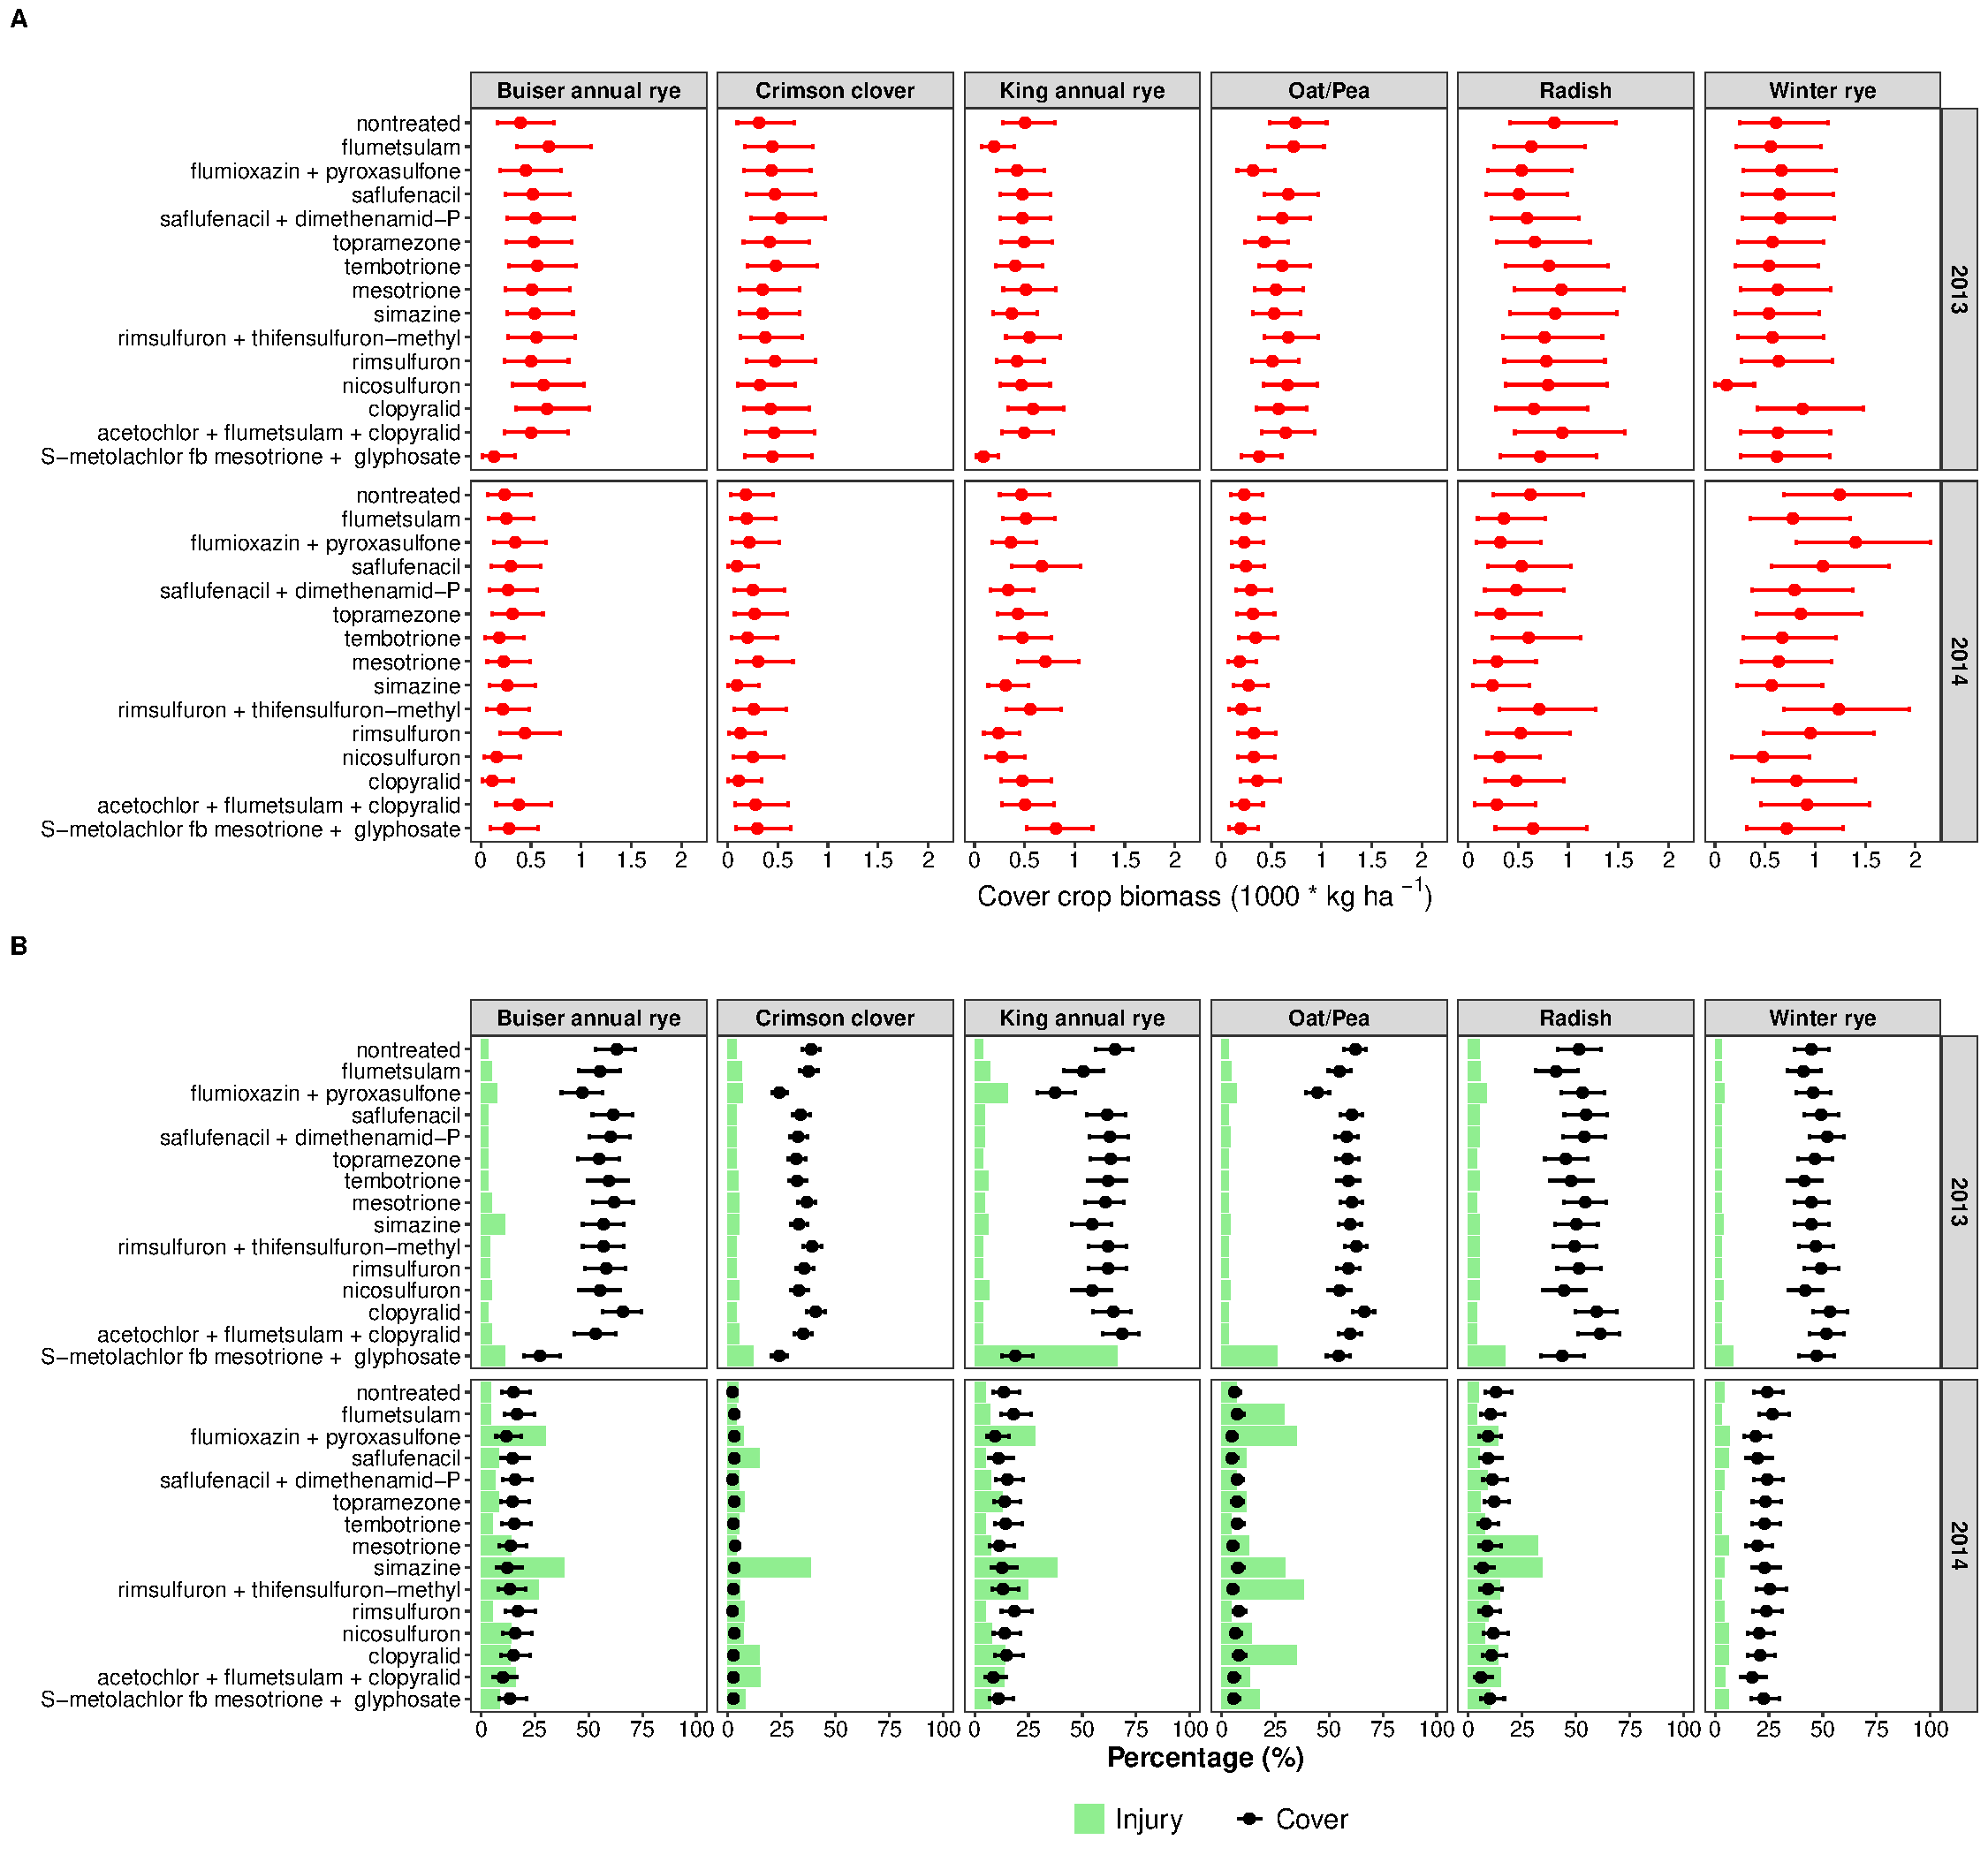
\includegraphics[width=17 cm]{CornF.pdf}
\caption{}
\end{figure}

\begin{figure}[H]
\centering
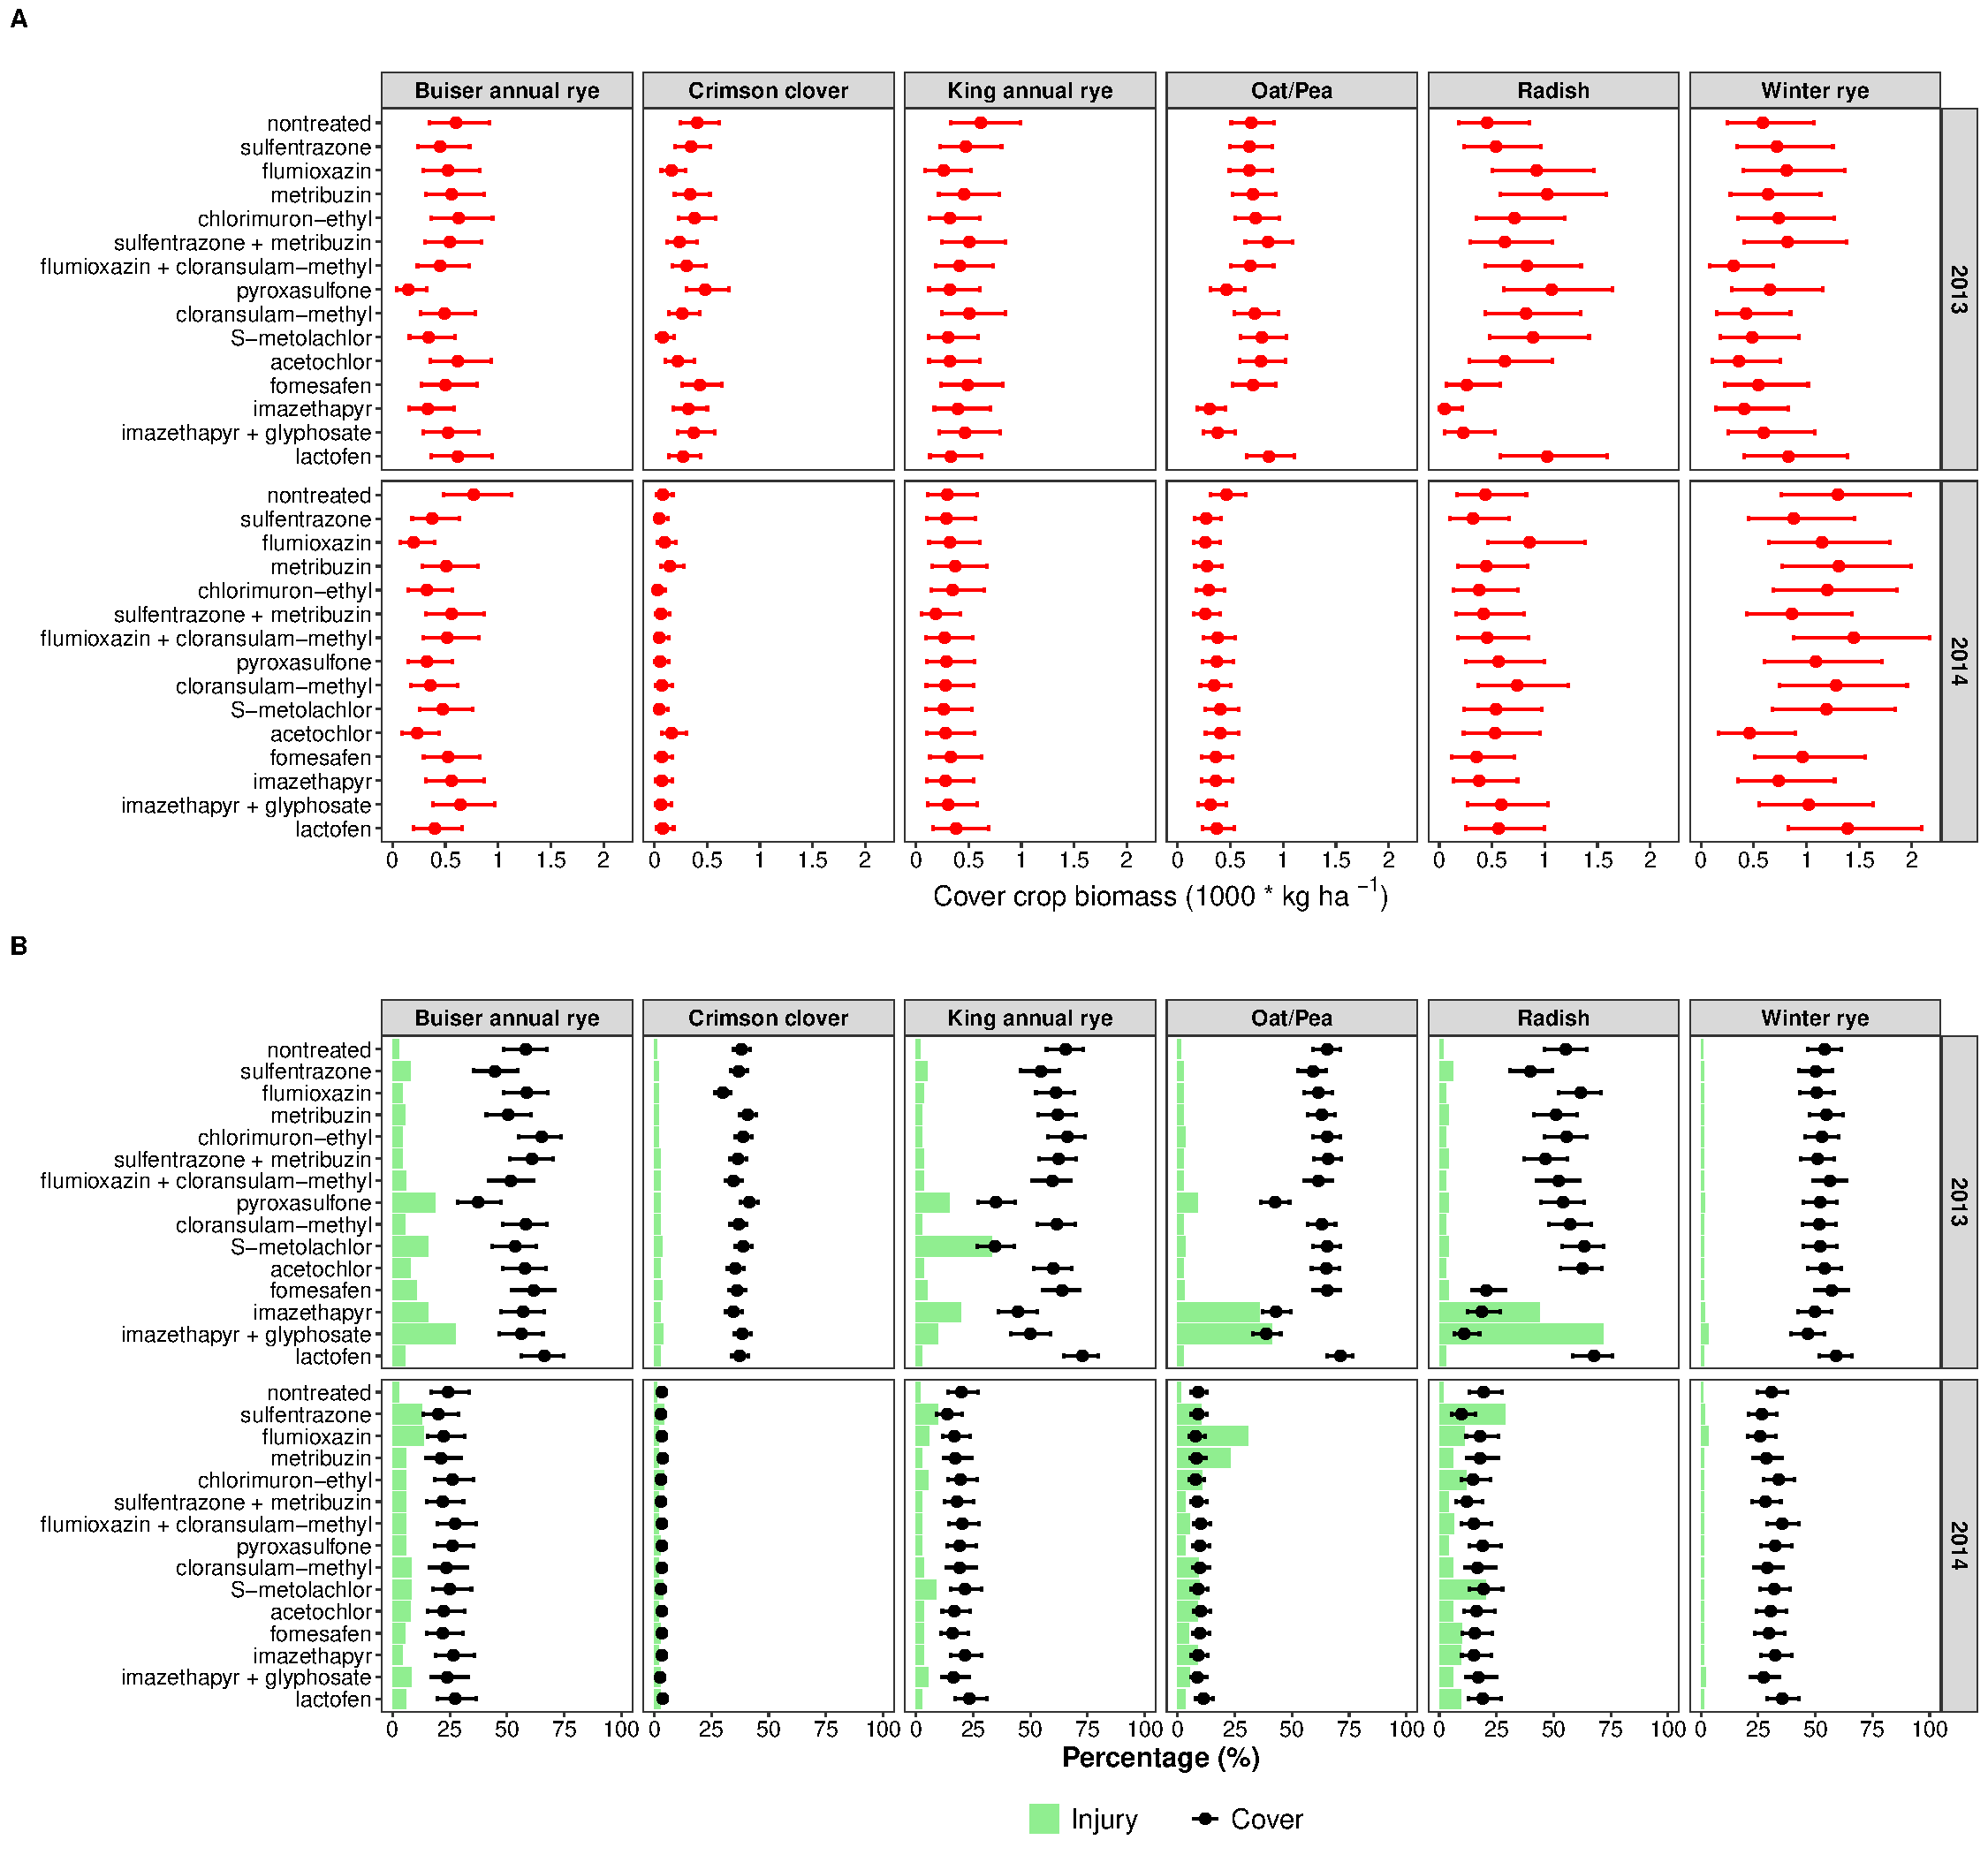
\includegraphics[width=17 cm]{SoyF.pdf}
\caption{}
\end{figure}

\hypertarget{discussion}{%
\section{Discussion}\label{discussion}}

\resizebox{\textwidth}{!}{%
  \begin{tabular}{llllllllllllll}
  \hline
  &              & \multicolumn{12}{c}{Species}                                                                                                                                                                                  \\ \cline{2-14} 
  Treatments                               &              & \multicolumn{2}{c}{Bruiser annual rye} & \multicolumn{2}{l}{Crimson clover} & \multicolumn{2}{l}{King annual rye} & \multicolumn{2}{l}{Oat/Pea} & \multicolumn{2}{l}{Radish} & \multicolumn{2}{l}{Winter rye} \\ \cline{3-14} 
  & Timing       & 2013               & 2014              & 2013             & 2014            & 2013             & 2014             & 2013         & 2014         & 2013         & 2014        & 2013           & 1014          \\ \hline
  &              & \multicolumn{12}{c}{------ Biomass (kg ha-1) ------}                                                                                                                                                          \\
  nontreated                               &              & 393                & 234               & 316              & 178             & 507              & 469              & 741          & 226          & 863          & 620         & 608            & 1242          \\
  flumetsulan                              & PRE          & 678                & 251               & 449              & 193             & 199              & 512              & 719          & 240          & 634          & 354         & 555            & 773           \\
  flumioxazin + pyroxasulfone              & PRE          & 446                & 339               & 433              & 216             & 428              & 362              & 319          & 232          & 535          & 321         & 665            & 1401          \\
  saflufenacil                             & PRE          & 515                & 303               & 468              & 90              & 474              & 670              & 670          & 243          & 506          & 530         & 649            & 1074          \\
  saflufenacil + demetenamid-P             & PRE          & 545                & 276               & 538              & 250             & 475              & 341              & 606          & 296          & 589          & 480         & 654            & 791           \\
  topramezone                              & EPOST        & 526                & 316               & 422              & 267             & 491              & 438              & 427          & 318          & 670          & 321         & 578            & 858           \\
  tembotrione                              & EPOST        & 564                & 188               & 483              & 203             & 410              & 480              & 606          & 342          & 806          & 602         & 538            & 668           \\
  mesotrione                               & EPOST        & 512                & 229               & 353              & 308             & 516              & 703              & 547          & 184          & 926          & 291         & 625            & 637           \\
  simazine                                 & EPOST        & 538                & 262               & 352              & 93              & 374              & 306              & 529          & 268          & 870          & 246         & 543            & 567           \\
  rimsulfuron + thifensulfuron-methyl      & EPOST        & 554                & 219               & 373              & 262             & 552              & 559              & 673          & 199          & 762          & 710         & 579            & 1233          \\
  rinsulfuron                              & EPOST        & 505                & 444               & 469              & 128             & 422              & 238              & 513          & 326          & 782          & 523         & 639            & 955           \\
  nicosulfuron                             & EPOST        & 622                & 160               & 323              & 248             & 471              & 277              & 663          & 324          & 800          & 315         & 118            & 476           \\
  clopyralid                               & EPOST        & 622                & 116               & 424              & 110             & 579              & 481              & 574          & 361          & 655          & 484         & 875            & 812           \\
  acetochlor + flumetsulam + clopyralid    & EPOST        & 501                & 378               & 460              & 275             & 495              & 501              & 642          & 231          & 935          & 287         & 625            & 919           \\
  S-metolachlor fb mesotrione + glyphosate & PRE fb LPOST & 129                & 283               & 444              & 292             & 94               & 815              & 374          & 196          & 719          & 650         & 622            & 720           \\ \hline
  Year                                     &              & 502                & 260               & 418              & 200             & 419              & 464              & 567          & 263          & 731          & 437         & 577            & 857           \\ \hline
  Anova                                    &              & \multicolumn{12}{c}{------ P-value ------}                                                                                                                                                                    \\ \cline{1-1}
  herbicide                                &              & \multicolumn{2}{l}{0.9189}             & \multicolumn{2}{l}{0.9218}         & \multicolumn{2}{l}{0.2809}          & \multicolumn{2}{l}{0.3490}  & \multicolumn{2}{l}{0.9082} & \multicolumn{2}{l}{0.0622}     \\
  year                                     &              & \multicolumn{2}{l}{0.0000}             & \multicolumn{2}{l}{0.0000}         & \multicolumn{2}{l}{0.2981}          & \multicolumn{2}{l}{0.0000}  & \multicolumn{2}{l}{0.0000} & \multicolumn{2}{l}{0.0003}     \\
  herbicide*year                           &              & \multicolumn{2}{l}{0.5099}             & \multicolumn{2}{l}{0.8989}         & \multicolumn{2}{l}{0.0065}          & \multicolumn{2}{l}{0.4091}  & \multicolumn{2}{l}{0.7519} & \multicolumn{2}{l}{0.8565}     \\ \hline
  \end{tabular}%
}

\textbackslash end\{table\}

Authors should discuss the results and how they can be interpreted in
perspective of previous studies and of the working hypotheses. The
findings and their implications should be discussed in the broadest
context possible. Future research directions may also be highlighted.

\hypertarget{conclusion}{%
\section{Conclusion}\label{conclusion}}

This section is not mandatory, but can be added to the manuscript if the
discussion is unusually long or complex.

\hypertarget{patents}{%
\section{Patents}\label{patents}}

This section is not mandatory, but may be added if there are patents
resulting from the work reported in this manuscript.

% %%%%%%%%%%%%%%%%%%%%%%%%%%%%%%%%%%%%%%%%%%
% %% optional
% \supplementary{The following are available online at www.mdpi.com/link, Figure S1: title, Table S1: title, Video S1: title.}
%
% % Only for the journal Methods and Protocols:
% % If you wish to submit a video article, please do so with any other supplementary material.
% % \supplementary{The following are available at www.mdpi.com/link: Figure S1: title, Table S1: title, Video S1: title. A supporting video article is available at doi: link.}

\vspace{6pt}

%%%%%%%%%%%%%%%%%%%%%%%%%%%%%%%%%%%%%%%%%%
\acknowledgments{All sources of funding of the study should be disclosed. Please clearly
indicate grants that you have received in support of your research work.
Clearly state if you received funds for covering the costs to publish in
open access.}

%%%%%%%%%%%%%%%%%%%%%%%%%%%%%%%%%%%%%%%%%%
\authorcontributions{For research articles with several authors, a short paragraph specifying
their individual contributions must be provided. The following
statements should be used ``X.X. and Y.Y. conceive and designed the
experiments; X.X. performed the experiments; X.X. and Y.Y. analyzed the
data; W.W. contributed reagents/materials/analysis tools; Y.Y. wrote the
paper.'' Authorship must be limited to those who have contributed
substantially to the work reported.}

%%%%%%%%%%%%%%%%%%%%%%%%%%%%%%%%%%%%%%%%%%
\conflictsofinterest{Declare conflicts of interest or state `The authors declare no conflict
of interest.' Authors must identify and declare any personal
circumstances or interest that may be perceived as inappropriately
influencing the representation or interpretation of reported research
results. Any role of the funding sponsors in the design of the study; in
the collection, analyses or interpretation of data in the writing of the
manuscript, or in the decision to publish the results must be declared
in this section. If there is no role, please state `The founding
sponsors had no role in the design of the study; in the collection,
analyses, or interpretation of data; in the writing of the manuscript,
an in the decision to publish the results'.}

%%%%%%%%%%%%%%%%%%%%%%%%%%%%%%%%%%%%%%%%%%
%% optional
\abbreviations{The following abbreviations are used in this manuscript:\\

\noindent
\begin{tabular}{@{}ll}
MDPI & Multidisciplinary Digital Publishing Institute \\
DOAJ & Directory of open access journals \\
TLA & Three letter acronym \\
LD & linear dichroism \\
\end{tabular}}

\input{"appendix.tex"}

%%%%%%%%%%%%%%%%%%%%%%%%%%%%%%%%%%%%%%%%%%
% Citations and References in Supplementary files are permitted provided that they also appear in the reference list here.

%=====================================
% References, variant A: internal bibliography
%=====================================
%\reftitle{References}
%\begin{thebibliography}{999}
% Reference 1
%\bibitem[Author1(year)]{ref-journal}
%Author1, T. The title of the cited article. {\em Journal Abbreviation} {\bf 2008}, {\em 10}, 142--149.
% Reference 2
%\bibitem[Author2(year)]{ref-book}
%Author2, L. The title of the cited contribution. In {\em The Book Title}; Editor1, F., Editor2, A., Eds.; Publishing House: City, Country, 2007; pp. 32--58.
%\end{thebibliography}

% The following MDPI journals use author-date citation: Arts, Econometrics, Economies, Genealogy, Humanities, IJFS, JRFM, Laws, Religions, Risks, Social Sciences. For those journals, please follow the formatting guidelines on http://www.mdpi.com/authors/references
% To cite two works by the same author: \citeauthor{ref-journal-1a} (\citeyear{ref-journal-1a}, \citeyear{ref-journal-1b}). This produces: Whittaker (1967, 1975)
% To cite two works by the same author with specific pages: \citeauthor{ref-journal-3a} (\citeyear{ref-journal-3a}, p. 328; \citeyear{ref-journal-3b}, p.475). This produces: Wong (1999, p. 328; 2000, p. 475)

%=====================================
% References, variant B: external bibliography
%=====================================
\reftitle{References}
\externalbibliography{yes}
\bibliography{mybibfile.bib}

%%%%%%%%%%%%%%%%%%%%%%%%%%%%%%%%%%%%%%%%%%
%% optional
\sampleavailability{Samples of the compounds \ldots\ldots{} are available from the authors.}

%% for journal Sci
%\reviewreports{\\
%Reviewer 1 comments and authors’ response\\
%Reviewer 2 comments and authors’ response\\
%Reviewer 3 comments and authors’ response
%}

%%%%%%%%%%%%%%%%%%%%%%%%%%%%%%%%%%%%%%%%%%
\end{document}

